\documentclass{beamer}
\usepackage[utf8]{inputenc}
\usetheme{Warsaw}

\title{Présentation CMMAI}
\author{H4203} %TODO

\begin{document}

\begin{frame}
\titlepage
\end{frame}

\begin{frame}
Introduction
\end{frame}

\begin{frame}
éventuelles spécifications venant compléter le sujet
TODO
\end{frame}

\begin{frame}
LSG simplifé de l'application globale avec le découpage en 3 lots fonctionnels
Schema LSG TODO
\end{frame}

\begin{frame}
IHM du poste distant
connection
\end{frame}

\begin{frame}
IHM du poste distant
configuration
\end{frame}

\begin{frame}
IHM du poste distant
log
\end{frame}

\begin{frame}
IHM du poste distant
erreur \/ warning
\end{frame}

\begin{frame}
\frametitle{Lot 1 : réseau, journalisation, gestion des évènements.}
    \begin{block}{Réalisé par Paul et Maxime}
	\begin{itemize}
	    \item   Communication réseau en entrée et en sortie du système.
	    \item   Communication des évènements par boite aux lettres à
	    l'intérieur du système.
	    \item   Gestion de la journalisation sur disque.
	\end{itemize}
    \end{block}
\end{frame}

\begin{frame}
\frametitle{Protocole}
    \begin{block}{Choix}
	\begin{itemize}
	    \item Protocole \texttt{plain text}.
	    \item Séparateur : retour chariot.
	    \item 9 commandes différentes dans les deux sens.
	\end{itemize}
    \end{block}
\end{frame}

\begin{frame}
\frametitle{Protocole en entrée}
\begin{enumerate}
		\item \texttt{RESUME} : reprise sur erreur.
		\item \texttt{STOP} : arrêt du système après les cartons courants.
		\item \texttt{CONFIG} : 5 valeurs chiffrées pour configurer le système.
		\item \texttt{LAUNCH} : lancer le système.
\end{enumerate}
\end{frame}

\begin{frame}
    \frametitle{LCG : Réseau, en entrée}
    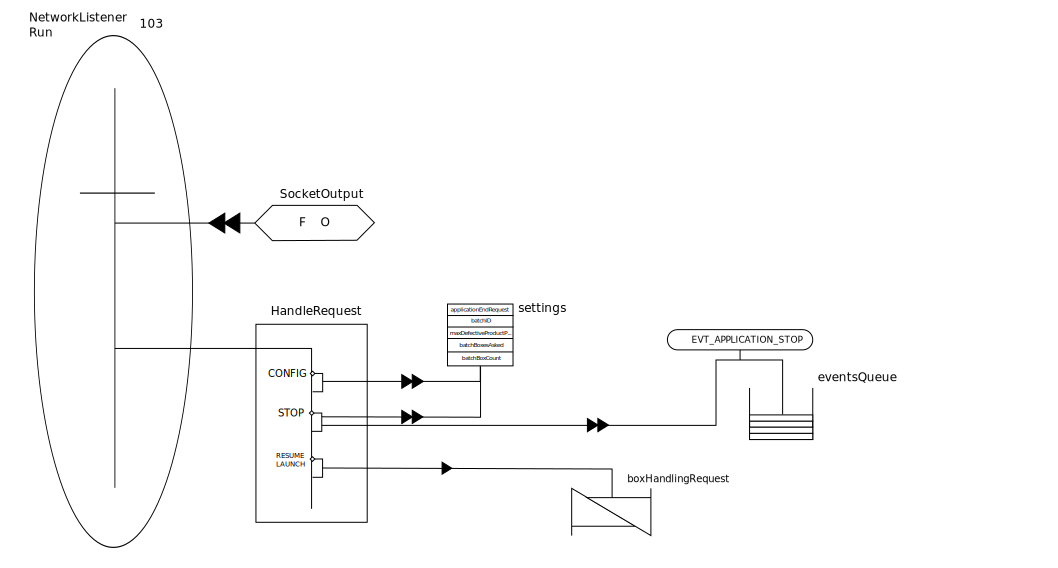
\includegraphics[width=\textwidth]{../SchemasLCG/NetworkListener-run.pdf}
\end{frame}

\begin{frame}
\frametitle{Protocole en sortie}
    \begin{enumerate}
		\item \texttt{REJECTED} : nombre de pièces ayant un défaut.
		\item \texttt{ACCEPTED} : un carton a été accepté par le système. Un argument pour indiquer le nombre de pièces.
		\item \texttt{LOG} : l'argument est un message à afficher.
		\item \texttt{ERROR} : erreur critique nécessitant une intervention. Un argument pour le code d'erreur.
		\item \texttt{WARNING} : erreur non critique (panne d'imprimante).
    \end{enumerate}
\end{frame}

\begin{frame}
    \frametitle{LCG : EventManager : réseau en sortie}
    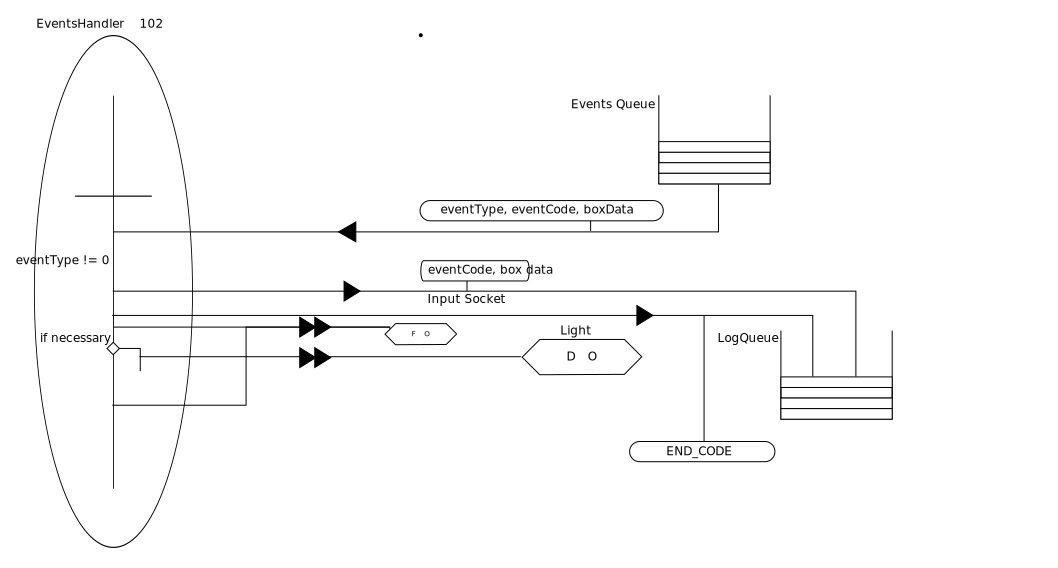
\includegraphics[width=\textwidth]{../SchemasLCG/src/EventsManager.pdf}
\end{frame}


\begin{frame}
    \frametitle{LCG : Journalisation sur disque}
    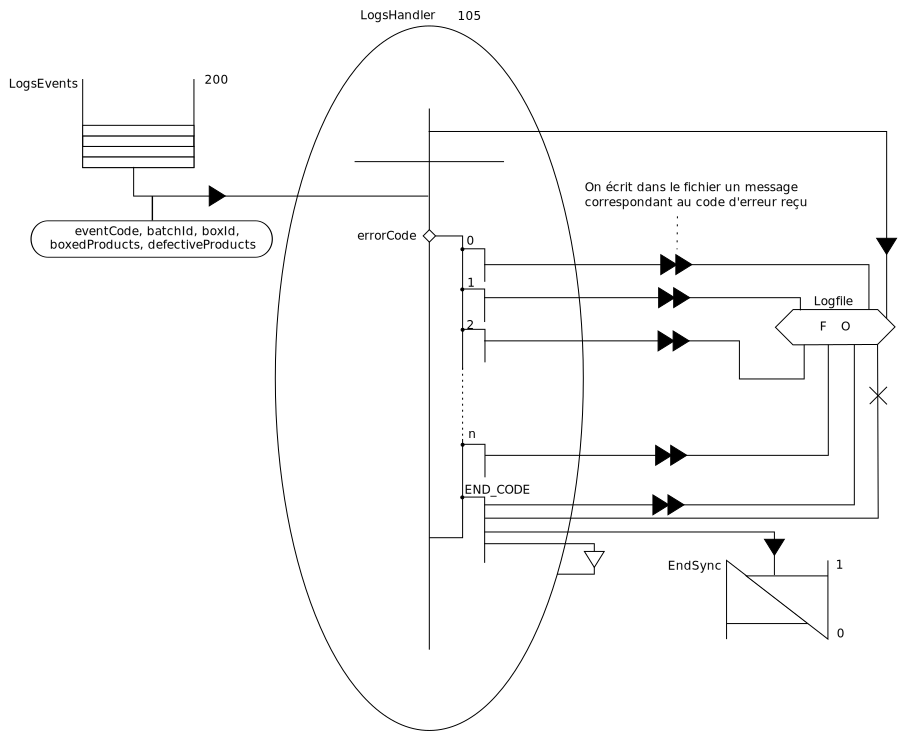
\includegraphics[width=\textwidth]{../SchemasLCG/LogsManager.pdf}
\end{frame}

\begin{frame}
Binôme 2
- LCG détaillé et complet en mode simulation
\end{frame}

\begin{frame}
Binôme 2
- justification des choix effectués pour la simulation  
\end{frame}

\begin{frame}
Binôme 3
- LCG détaillé et complet en mode simulation
\end{frame}

\begin{frame}
Binôme 3
- justification des choix effectués pour la simulation 
\end{frame}

\begin{frame}
- Intégration (démarche, plan, tests, resultats)
%TODO
\end{frame}

\begin{frame}
- démonstration de vos réalisations
démonstration externe au slides ?
\end{frame}

\begin{frame}
- bilan du projet (auto-critique, améliorations possibles, points forts/faibles, difficultés rencontrées ...) 
%TODO
\end{frame}
\end{document}

